\section{The importance of reductions}
A reduction in terms of parallel programming is an operation, where a large dataset of entries (e.g. numbers) is reducted to one entry.
The simplest example is the sum of a set of numbers and will be used for the rest of this work.
More generally are reduction is defined by an operation \( \circ: X \times X \rightarrow X \) on two entries with the following properties:
\begin{align}
    a \circ b &= b \circ a \ \ \mathrm{(commutativity)}, \\
    a \circ (b \circ c) &= (a \circ b) \circ c \ \ \mathrm{(associativity)}.
\end{align}
This guarantees that the result is (mathematically) independent of the order in which the elements are reduced.
Note, that these properties do not ensure numerical stablility.

The reduction operation, first and foremost the sum, plays a crucial role in all of numerics.
Simple linear algebra operations like the scalar product or the matrix multiplication already include a reduction:
The entries of two vectors are multiplied element wise and the summed up.
In machine learning, reductions are present as a key step in feed-forward networks:
Again all the values of the node one layer below are multiplied by weights elementwise and the summed up to calculated the value of a singular node above.
Reductions are a very basic and fundamental operation and, therefore, an efficient implementation is required. 

\section{The tree reduction algorithm}
\begin{figure}
    \centering
    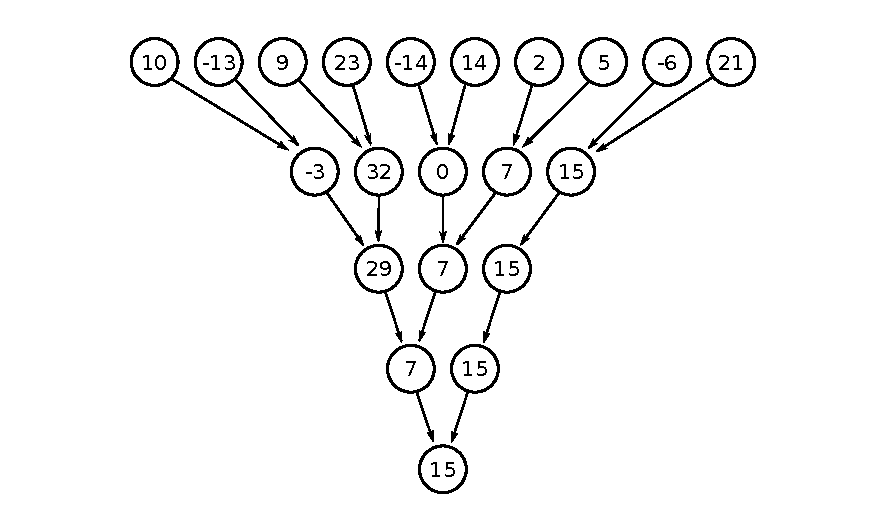
\includegraphics{tree_reduction.pdf}
    \caption{
        Example of a tree reduction of ten elements.
        Note how there is a leftover after the first reduction.
        These are usually handled by zeropadding (i.e. adding zeros) after each step to make the number of elements divisible by 2.
    }
\end{figure}
The most efficient (shortest execution time) algorithm is heavily dependent on the underlying hardware.
For example, a node network with a lot of parallelisation overhead and a complicated communication topology might use a ring algorithm ("add value and pass to next thread/node").
In this work the focus is on single GPU reductions.
Here, the tree reduction approach is the most successful.
All available threads are called to reduce two entries to one in parallel, effectively halving the size of the dataset in one step.
This is repeated until only one entry remains.

\section{Naive implementation with CUDA}
For a better understanding of the CUDA framework and tree reduction algorithm an unoptimized code is presented which implements the algorithm for the case of addition of signed 32-bit integers. 
Note, that even though this is unoptimized GPU code, it runs magnitudes faster than on a CPU (exact speedup depending on the problem size and the available hardware).

When approaching a problem using CUDA the big challenge is to map the for-loop that one wants to parallelize to blocks and CUDA-threads. 
Often, the best starting point is to write serial CPU code to get a feeling for the problem and to have a working solution to test the optimized solutions against later.
In this case, we will first implement a serial tree reduction in C and port this code to CUDA in a second step.

\subsection{Serial tree reduction on a CPU}
\begin{figure} \label{fig_naive_reduction}
    \centering
    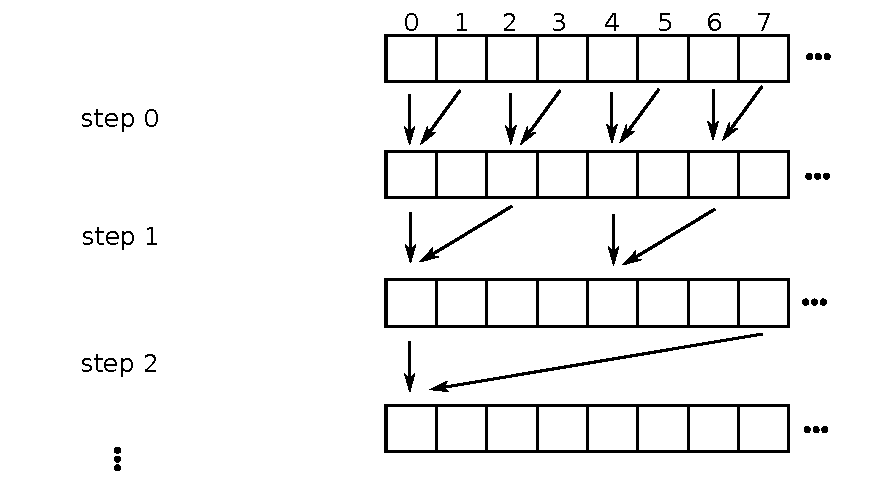
\includegraphics{naive_reduction.pdf}
    \caption{
        Sketch of the implementation of the tree reduction algorithm presented in this section.
        The cells denote entries in the data array.
        Two arrows pointing into a cell denote addition of the source cells values and writing of the result into the target cell.
        The final result is found in the first cell of the array.
    }
\end{figure}
Our starting point is an integer array \texttt{h\_in}.
The \texttt{h\_} denotes data stored on the host (CPU RAM), which is a useful convention, since CUDA does not distinguish between pointers to host and device memory.
For simplicity, we assume that the size of the array is a power of two.
If this is not the case, one could simply zeropad the data and would still be able to use the code.

Let's write a function \texttt{reduce} that executes the tree reduction.
This function takes an input array \texttt{h\_in}, performs the reduction and writes the result to an output \texttt{h\_out}. 
We need two for-loops:
One to iterate over the step of the reduction (vertically in Fig. \ref{fig_naive_reduction}) and one to iterate over the (remaining) data set (horizontally). 
A temporary array is used to perform the reduction on, so the input array stays untouched.

\lstinputlisting[language=C]{code/host_reduce.c}

Note that the \texttt{memcpy} function call could be avoided, but ports nicely to GPU code later on, which is the reason why it was used.
The inner loop of this implementation could be parallelised easily, since each step of the inner loop is independent.
This means, however, that with each step of the outer loop all threads are created and destroyed, which leads to a large parallelisation overhead.
While this parallelisation overhead can be avoided on CPUs using persistant threads, there is another solution that ports nicely to GPU code later on.
The outer loop cannot be parallelized, since each step is dependent on the result of the step before.
To fix this, one can swap the two loops.
While this requires slightly more code, it greatly simplifies all examples in the following.
The rewritten function looks like this:

\lstinputlisting[language=C]{code/host_reduce_swapped_loops.c}

Note that an additional if-statement is required.
This is a much better basis for parallelisation, since now the outer loop can be parallelised.
However, one needs to be very careful as this is now prone to a race-condition.
The parallelisation with CUDA is done in the next section.

It should be noted, that there are much faster ways to implement a reduction algorithm as a single-thread CPU application.
This code has been written with the intent of parallelisation on a GPU and serves solely this purpose.

\subsection{Tree reduction in CUDA for small arrays}
Once the algorithm has been successfully implemented serially, the parallelisation of the target for-loop is always the same.
One needs to map the domain of the for-loop (here integers from \texttt{0} to \texttt{len-1}) to threads.
The maximum number of threads \( n_{\mathrm{Threads}} \) a block can contain depends on the hardware, but is always a power of two.
Nvidia GPUs with compute capability of 2.0 or higher will allow for \( n_{\mathrm{Threads}} = 1024 \) (e.g. RTX 30xx series and A100, see \cite{programming_guide}), but it is not necessarily optimal to use all threads.
This will be explored later.
For now we will restrict the maximum size of our input array to 1024, such that only one block is required.
With this, one can write down the kernel (terminology for a function running on the GPU).

\lstinputlisting[language=C]{code/device_small_kernel0.cu}

There are several things to uncover here. First, the \texttt{\_\_global\_\_ void} declares the function as a kernel, which runs on the device but can be invoked from the host. 
Secondly there is a new constant \texttt{threadIdx.x} available within the kernel.
This is an identifier of the thread that is executing the kernel.
It is unique for all threads within a block and ranges from \texttt{0} to \texttt{numThreadsPerBlock - 1}.
This replaces the index which the for-loop iterated over.
The temporary array can be replaced by the ultra-fast cache shared by all threads of one block, which is allocated during kernel invocation and declared within the kernel by the line

\lstset{firstnumber = 5}
\lstinputlisting[language=C]{code/shared_memory_line.cu}
\lstset{firstnumber = 1}

As mentioned earlier, there is a race condition between threads, which can be solved by the \texttt{\_\_syncthreads()} method.
This method acts as a wait-for-all barrier within a block (synchronisation between blocks is not possible!).
Finally, the result needs to be exported.
For this, only one thread is required, hence the if-statement.
Note that the input and output pointer names start with a \texttt{d\_}, which is not required but is a convention to mark, that these pointers live in the adress space of the device.

The kernel can be invoked from the host with the following code:

\lstinputlisting[language=C]{code/kernel_invokation.cu}

First the data is copied to the device memory.
Then the kernel is invoked by the triple angled brackets syntax.
Within the brackets, the number of blocks \( n_\mathrm{Blocks} \) (so far exactly one), the number of threads per block \( n_{\mathrm{Threads}} \) and the amount of cache space are specified.
The kernel arguments are specified in parenthesis.
Finally the result is copied back to the host and the device memory is free'd.
Note that in practice one would write more code to error-check every step, assure that the correct upstream is used and optimize the copy procedure.
Nontheless, this is a minimal working example.

The big problem with this implementation is, that it is limited to an array size of 1024, since we only use one block.
This is solved in the next section.


\subsection{Tree reduction in CUDA for arbitrary array sizes}
\begin{figure}
    \centering
    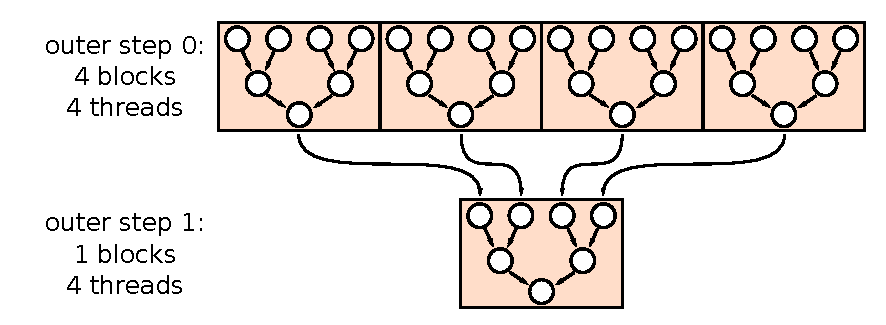
\includegraphics{block_reduction.pdf}
    \caption{
        Depicted is the schematic tree reduction in block structure for an array of length 16 and 4 threads per block.
        The first step requires 4 blocks and the second 1 block.
        The blocks run on the SMs of the GPU.
        The first step allows for four SMs and a total of 16 physical threads to be used in parallel.
        Between the two steps the output array is used as new input array.
        The second step can only make use of a single SM.
    }
\end{figure}
The limitation to an array size \( n_{\mathrm{Data}}\) of maximum block size can be solved in the following way:
Split the array into equal chunks and run the kernel on each of these chunks individually.
This procedure returns an array with size \( n_{\mathrm{Data}}/ n_{\mathrm{Threads}} \) (assuming that \( n_{\mathrm{Data}} \) is a power of 2, otherwise round up is required).
The procedure is then again used recursively, until the array is reduced to a singular value.
We refer to such a reduction step as "outer step", which reduces \( n_{\mathrm{Threads}} \) elements, compared to an "inner step" reducing 2 elements.

While this could be implemented already with the existing kernel, there is a hardware structure available to do kernel invokations with a certain amount of threads in parallel, namely the streaming multiprocessors (SMs).
The SMs are a second layer of parallelisation.
One block of threads is always mapped to one SM, so several blocks can be executed in parallel on several SMs.
Unlike the number of threads per block, the number of blocks is unlimited and blocks are queued until a SM is free to work on it.
In our case this has the following implication.
Lets assume that the initial array size is \( n_{\mathrm{Data}} = n \times 1024 \).
Then one could use \( n \) blocks of 1024 threads to do the first step of the outer reduction and use the full computational power of the GPU this way.

This leaves us with a new problem, however.
Namely, how does one calculate the position of the array one specific thread is supposed to work on?
To this end, CUDA offers two more constants in the kernel:
\texttt{blockDim.x} and \texttt{blockIdx.x}.
The first one is simply the number of threads in a block and the second one is a unique identifier of the current block, ranging from 0 to \( n_{\mathrm{Blocks}} - 1\).
The array position can then be calculated with \texttt{threadIdx.x + blockIdx.x * blockDim.x}.
The required amount of blocks for the kernel invokation can be calculated with rounding up division.
This can be neatly done with \( n_{\mathrm{Blocks}} = (n_{\mathrm{Data}} + n_{\mathrm{Threads}} - 1) / n_{\mathrm{Threads}} \), where the "\( / \)" denotes integer division.

To enable the use of blocks with our kernel three small modifications need to be done.
First, the access of our input array needs to be rewritten with the new formula for the position.
Secondly, the output is not a singular value but an array.
Thirdly, the range of the loop and the input array length can be deduced directly from the block size and number of threads per block and, therefore, the length of the input array does not need to be passed to the kernel.
The result from the \(i\)-th block should be written into the \(i\)-th position.
Also for simplicity the loop over the \texttt{step}-variable has been replaced by a loop over \texttt{stride} directly, saving an extra variable and the \texttt{log2} function call.
The finished code looks like this:

\lstinputlisting[language=C]{code/device_full_kernel0.cu}

The invokation changes slightly.
First, we need to specify the number of required blocks as argument in the triple angled brackets.
Secondly, the kernel has only two arguments now.
Also the size of the output array changes.

\lstinputlisting[language=C]{code/kernel_invokation_full.cu}

Note that this code only executes a single outer step of the reduction.
One would need to take the output array and feed it through this code until a single value is left.
This was left out since it is mostly host code and not of particular interest for the rest of the work.
It should be noted, however, that all code timings in the following were done for the full reduction.

\section{Conclusion}
This concludes the introduction to CUDA and tree reduction algorithms.
From now on this work focuses on modifying the kernel to optimize it as much as possible.
It should be noted, that a lot of optimization has been done already.
For example, using the explicitly declared shared memory instead of DRAM or the implementation of the block structure already offer a great speedup compared to other algorithms one could come up with.
Now, the main goal is to dive deeper into the hardware structure and achieve speedups by fixing problems like warp divergence and memory bank conflicts, which will be explained in full detail.
Some algorithmic improvements will also be done and in the end all the optimisations will be benchmarked on several hardware systems.
